\documentclass[10pt]{article}
\usepackage[polish]{babel}
\usepackage[utf8]{inputenc}
\usepackage[T1]{fontenc}
\usepackage{amsmath}
\usepackage{amsfonts}
\usepackage{amssymb}
\usepackage[version=4]{mhchem}
\usepackage{stmaryrd}
\usepackage{bbold}
\usepackage{graphicx}
\usepackage[export]{adjustbox}
\graphicspath{ {./images/} }

\title{PRACA KONTROLNA nr 1 - POZIOM PODSTAWOWY }

\author{}
\date{}


\begin{document}
\maketitle
\begin{enumerate}
  \item Wzrost kursu Euro w stosunku do złotego spowodował podwyżkę ceny nowego modelu Volvo o $5 \%$. Ponieważ nie było popytu na te samochody, więc postanowiono ustalić cenę promocyjną na poziomie odpowiadającym wzrostowi kursu Euro o 2\%.\\
a) O ile procent cena promocyjna była niższa od ceny wynikającej z faktycznego wzrostu kursu Euro w stosunku do złotego? Wynik podać z dokładnością do 1 promila.\\
b) Ile pan Kowalski stracił na wzroście kursu Euro, a ile zyskał dzięki cenie promocyjnej, jeżeli kupił samochód za 56000? Rachunki prowadzić z dokładnością do całkowitych złotych.
  \item Z obozu A do obozu B można przejść drogą żwirową lub ścieżką przez las, która jest o sześć kilometrów krótsza niż droga żwirowa. Bolek wyszedł z A i idąc ścieżką z prędkością $4 \mathrm{~km} / \mathrm{h}$ dotarł do B 1 godzinę wcześniej niż Lolek, który w tym samym momencie wyruszył drogą żwirową. Znaleźć długość ścieżki, wiedząc, że prędkość, z jaką porusza się Lolek wyraża się liczbą całkowitą.
  \item Ile jest naturalnych liczb pięciocyfrowych, w których zapisie dziesiętnym występują dokładnie dwa 0 i dokładnie jedna cyfra 1 ?
  \item Niech $A=\left\{x \in \mathbb{R}: \frac{1}{x^{2}+2} \geqslant \frac{1}{6-3 x}\right\}$ oraz $B=\{x \in \mathbb{R}:|x-2|+|x+2|<6\}$. Znaleźć i zaznaczyć na osi liczbowej zbiory $A, B$ oraz $(A \backslash B) \cup(B \backslash A)$.
  \item Uprościć wyrażenie
\end{enumerate}

$$
\frac{1}{\sqrt[6]{a^{5}}-\sqrt[6]{a^{2} b^{3}}}\left(\sqrt[6]{a^{5}}-\frac{b}{\sqrt[6]{a}}\right)-\frac{a-b}{a+\sqrt{a b}}
$$

dla $a, b$, dla których ma ono sens, a następnie obliczyć jego wartość, przyjmując $a=4-2 \sqrt{3}$ i $b=3+2 \sqrt{2}$.\\
6. Grupa 175 robotników firmy pana Kowalskiego miała wykonać pewien odcinek autostrady A4 w określonym terminie. Po upływie 30 dni wspólnej pracy okazało się, że musi możliwie szybko dokonać naprawy oddanego wcześniej odcinka autostrady A2. W związku z tym codziennie odsyłano do tego zadania kolejnych 3 robotników, wskutek czego prace przy budowie autostrady A4 zakończono z 21-dniowym opóżnieniem. W jakim czasie planowano pierwotnie wybudować dany odcinek autostrady A4?

\section*{PRACA KONTROLNA nr 1 - POZIOM ROZSZERZONY}
\begin{enumerate}
  \item Pan Kowalski zaciągnął 31 grudnia pożyczkę 4000 złotych oprocentowaną w wysokości $18 \%$ w skali roku. Zobowiązał się spłacić ją w ciągu roku w trzech równych ratach płatnych 30 kwietnia, 30 sierpnia i 30 grudnia. Oprocentowanie pożyczki liczy się od 1 stycznia, a odsetki od kredytu naliczane są w terminach płatności rat. Obliczyć wysokość tych rat w zaokraggleniu do pełnych groszy.
  \item Z dwu stacji wyjeżdżają jednocześnie naprzeciw siebie dwa pociągi. Pierwszy jedzie z prędkością $15 \mathrm{~km} / \mathrm{h}$ większą niż drugi i spotykają się po 40 minutach. Gdyby drugi pociąg wyjechał o 9 minut wcześniej, to, jadąc z tymi samymi prędkościami, spotkałyby się w połowie drogi. Znaleźć odległość między miejscowościami oraz prędkości każdego z pociągów.
  \item Ile jest liczb pięciocyfrowych podzielnych przez 9, które w rozwinięciu dziesiętnym mają: a) obie cyfry 1,2 i tylko te? b) obie cyfry 2,3 i tylko te? c) wszystkie cyfry $1,2,3$ i tylko te? Odpowiedź uzasadnić.
  \item Narysować na płaszczyźnie zbiór $A=\left\{(x, y): \sqrt{-2 x-x^{2}} \leqslant y \leqslant \sqrt{3}|x+1|\right\}$ i obliczyć jego pole.
  \item Uprościć wyrażenie ( dla $a, b$, dla których ma ono sens)
\end{enumerate}

$$
\left(\frac{\sqrt[6]{b}}{\sqrt{b}-\sqrt[6]{a^{3} b^{2}}}-\frac{a}{\sqrt{a b}-a \sqrt[3]{b}}\right)\left[\frac{\sqrt[6]{a}}{\sqrt{b}\left(\sqrt[6]{a^{5}}-\sqrt[3]{a} \sqrt{b}\right)}\left(\sqrt[6]{a^{5}}-\frac{b}{\sqrt[6]{a}}\right)-\frac{\sqrt[6]{a}(a-b)}{a \sqrt{b}+b \sqrt{a}}\right],
$$

a następnie obliczyć jego wartość dla $a=6 \sqrt{3}-10 \quad$ i $\quad b=10+6 \sqrt{3}$.\\
6. Dwaj turyści wyruszyli jednocześnie: jeden z punktu $A$ do punktu $B$, drugi - z $B$ do $A$. Każdy z nich szedł ze stałą prędkością i dotarłszy do mety, natychmiast ruszał w drogę powrotną. Pierwszy raz minęli się w odległości 12 km od punktu $B$, drugi - po upływie 6 godzin od momentu pierwszego spotkania - w odległości 6 km od punktu $A$. Obliczyć odległość punktów $A$ i $B$ i prędkości, z jakimi poruszali się turyści.

\section*{PRACA KONTROLNA nr 2 - POZIOM PODSTAWOWY}
\begin{enumerate}
  \item Rozwiązać nierówność $x^{3}+n x^{2}-m^{2} x-m^{2} n \leqslant 0$, gdzie
\end{enumerate}

$$
m=\frac{64^{\frac{1}{3}} \sqrt{2}+8^{\frac{1}{3}} \sqrt{64}}{\sqrt[3]{64 \sqrt{8}}} \quad \text { oraz } \quad n=\frac{(\sqrt{2})^{-4}\left(\frac{1}{4}\right)^{-\frac{5}{2}} \sqrt[4]{3}}{(\sqrt[4]{16})^{3} \cdot 27^{-\frac{1}{4}}}
$$

\begin{enumerate}
  \setcounter{enumi}{1}
  \item Dla jakich wartości $\alpha \in[0,2 \pi]$ liczby $\sin \alpha, 6 \cos \alpha, 6 \operatorname{tg} \alpha$ tworzą ciąg geometryczny?
  \item Suma pewnej ilości kolejnych liczb naturalnych równa jest 33, a różnica kwadratów największej i najmniejszej wynosi 55 . Wyznaczyć te liczby.
  \item Narysować wykres funkcji
\end{enumerate}

$$
f(x)=\left\{\begin{array}{lll}
x^{2}-6|x|+5, & \text { gdy } & |x-2| \leqslant 3 \\
|x-2|-3, & \text { gdy } & |x-2|>3
\end{array}\right.
$$

i wyznaczyć zbiór jej wartości. Dla jakich argumentów $x$ wykres funkcji $f(x)$ leży pod prostą $x-2 y+10=0$ ? Zilustrować rozwiązanie graficznie.\\
5. Dla jakiego parametru $m$ równanie $x^{2}-m x+m^{2}-2 m+1=0$ ma dwa różne pierwiastki w przedziale $(0,2)$ ?\\
6. Wierzchołek $A$ wykresu funkcji $f(x)=a x^{2}+b x+c$ leży na prostej $x=3$ i jest odległy od początku układu współrzędnych o 5 . Pole trójkąta, którego wierzchołkami są punkty przecięcia wykresu z osią $O x$ oraz punkt $A$ równe jest 8 . Podać wzór funkcji, której wykres jest obrazem paraboli $f(x)$ w symetrii względem punktu $(1, f(1))$.

\section*{PRACA KONTROLNA nr 2 - POZIOM ROZSZERZONY}
\begin{enumerate}
  \item Obliczyć $a$ wiedząc, że liczba $\left[\frac{2+9 \sqrt{2}}{2 \sqrt{2}-2}-\frac{1}{2}(2+\sqrt{2})^{2}\right]-\left(\frac{\sqrt[6]{32}}{2 \sqrt{2}-2}\right)^{3}$ jest miejscem zerowym funkcji $f(x)=2^{x}-a^{3} x$.
  \item Dziesiąty wyraz rozwinięcia $\left(\frac{1}{\sqrt{x}}-\sqrt[3]{x}\right)^{n}$ nie zawiera $x$. Wyznaczyć współczynniki przy najniższej i najwyższej potędze $x$.
  \item Wyznaczyć zbiór wartości funkcji $f(x)=\left(\log _{2} x\right)^{3}+\log _{2} \frac{x^{2}}{4}-1$ na przedziale $(1,2)$.
  \item Tangens kąta ostrego $\alpha$ równy jest $\frac{a}{7 b}$, gdzie
\end{enumerate}

$$
a=(\sqrt{2}+1)^{3}-(\sqrt{2}-1)^{3}, \quad b=(\sqrt{\sqrt{2}+1}-\sqrt{\sqrt{2}-1})^{2}
$$

Wyznaczyć wartości pozostałych funkcji trygonometrycznych tego kąta oraz kąta $2 \alpha$. Jaka jest miara kąta $\alpha$ ?\\
5. Trzy liczby $x<y<z$, których suma jest równa 93 tworzą ciąg geometryczny. Te same liczby można uważać za pierwszy, drugi i siódmy wyraz ciągu arytmetycznego. Jakie to liczby?\\
6. Określić liczbę pierwiastków równania $(2 m-3) x^{2}-4 m|x|+m-1=0$ w zależności od parametru $m$.

\section*{PRACA KONTROLNA nr $\mathbf{3}$ - POZIOM PODSTAWOWY}
\begin{enumerate}
  \item Wektory $\overrightarrow{A B}=[2,2], \overrightarrow{B C}=[-2,3], \overrightarrow{C D}=[-2,-4]$ są bokami czworokąta $A B C D$. Punkty $K$ i $M$ są środkami boków $C D$ oraz $A D$. Obliczyć pole trójkąta $K M B$ oraz jego stosunek do pola całego czworokąta. Sporządzić rysunek.
  \item Narysować wykres funkcji
\end{enumerate}

$$
f(x)=\frac{1}{\sqrt{1+\operatorname{tg}^{2} x}}-\frac{1}{2}
$$

a następnie rozwiązać graficznie nierówność $f(x)<0$.\\
3. Rozwiązać nierówność $w(x-2)>w(x-1)$, gdzie

$$
w(x)=x^{4}-4 x^{3}+5 x^{2}-2 x
$$

\begin{enumerate}
  \setcounter{enumi}{3}
  \item Tangens kąta ostrego $\alpha$ równy jest
\end{enumerate}

$$
\sqrt{7-4 \sqrt{3}}
$$

Wyznaczyć wartości pozostałych funkcji trygonometrycznych tego kąta. Wykorzystując wzór $\sin 2 \alpha=2 \sin \alpha \cos \alpha$ wyznaczyć miarę kąta $\alpha$.\\
5. Punkt $B(2,6)$ jest wierzchołkiem trójkąta prostokątnego o polu 25 , którego przeciwprostokątna zawarta jest w prostej $x-2 y=0$. Obliczyć wysokość opuszczoną na przeciwprostokątną i wyznaczyć współrzędne pozostałych wierzchołków trójkąta.\\
6. Dane są punkty $A(-1,-3)$ i $B(2,-2)$. Na paraboli $y=x^{2}-1$ znaleźć taki punkt $C$, aby pole trójkąta $A B C$ było najmniejsze.

\section*{PRACA KONTROLNA nr 3 - POZIOM ROZSZERZONY}
\begin{enumerate}
  \item Dla jakich wartości parametru $\alpha \in(0,2 \pi)$ funkcja
\end{enumerate}

$$
f(x)=\sin \alpha \cdot x^{2}-x+\cos \alpha
$$

posiada minimum lokalne i wartość najmniejsza funkcji jest ujemna?\\
2. Rozwiązać równanie

$$
\sqrt{3}+\operatorname{tg} x=4 \sin x
$$

\begin{enumerate}
  \setcounter{enumi}{2}
  \item Wielomian $w(x)=x^{4}+3 x^{3}+p x^{2}+q x+r$ dzieli się przez $x-2$, a resztą z jego dzielenia przez $x^{2}+x-2$ jest $-4 x-12$. Wyznaczyć współczynniki $p, q, r$ i rozwiązać nierówność $w(x) \geqslant 0$.
  \item W czworokącie $A B C D$ dane są $A D=a$ oraz $A B=2 a$. Wiadomo, że $\overrightarrow{A C}=2 \overrightarrow{A B}+3 \overrightarrow{A D}$ oraz $\angle B A D=60^{\circ}$. Stosując rachunek wektorowy obliczyć cosinus kąta $A B C$ oraz obwód czworokąta. Rozwiązanie zilustrować rysunkiem.
  \item Punkt $P\left(-\sqrt{3}, \frac{\sqrt{3}}{2}\right)$ jest środkiem boku trójkąta równobocznego. Drugi bok trójkąta leży na prostej $y=2 x$. Wyznaczyć współrzędne wszystkich wierzchołków trójkąta i obliczyć jego pole. Sporządzić rysunek.
  \item Wyznaczyć zbiór punktów płaszczyzny utworzonych przez środki wszystkich okręgów stycznych jednocześnie do prostej $y=0$ oraz do okręgu $x^{2}+y^{2}-4 y+3=0$. Sporządzić rysunek.
\end{enumerate}

\section*{PRACA KONTROLNA nr 4 - POZIOM PODSTAWOWY}
\begin{enumerate}
  \item Na półkuli o promieniu $r$ opisano stożek o kącie rozwarcia $2 \alpha \mathrm{w}$ taki sposób, że środek podstawy stożka znajduje się w środku półkuli. Oblicz objętość i pole powierzchni stożka. Jaki jest stosunek objętości stożka do objętości półkuli dla kąta rozwarcia $\pi / 3$ ?
  \item Kula jest styczna do wszystkich krawędzi czworościanu foremnego o krawędzi $a$. Oblicz promień tej kuli.
  \item W kwadrat $A B C D$ wpisano kwadrat $E F G H$, który zajmuje $3 / 4$ jego powierzchni. W jakim stosunku wierzchołki kwadratu $E F G H$ dzielą boki kwadratu $A B C D$ ?
  \item Niech $f(x)=4^{x+4}-7 \cdot 3^{x+3}$ i $g(x)=6 \cdot 4^{4 x}-3^{4 x+2}$.
\end{enumerate}

Rozwiąż nierówność $f(x-3) \leqslant g\left(\frac{x}{4}\right)$.\\
5. Znajdź wymiary trapezu równoramiennego o obwodzie $d$ i kącie ostrym przy podstawie $\alpha$ o największym polu.\\
6. W trójkąt równoboczny o boku $a$ wpisujemy trójkąt, którego wierzchołkami są środki boków naszego trójkąta. Wpisany trójkąt kolorujemy na niebiesko. Następnie w każdy z niepokolorowanych trójkątów wpisujemy w ten sam sposób kolejne niebieskie trójkąty, itd. Znajdź sumę pól niebieskich trójkątów po $n$ krokach. Po ilu krokach niebieskie trójkąty zajmą co najmniej $50 \%$, a po ilu - $75 \%$ powierzchni wyjściowego trójkąta?

\section*{PRACA KONTROLNA nr 4 - POZIOM ROZSZERZONY}
\begin{enumerate}
  \item W trójkącie prostokątnym $A B C$ dane są przyprostokątne $|A C|=3$ oraz $|C B|=4$. Punkt $D$ jest spodkiem wysokości opuszczonej z wierzchołka kąta prostego, a $E$ i $F$ punktami przecięcia przeciwprostokątnej z dwusiecznymi kątów $A C D$ i $D C B$. Oblicz długość odcinka $E F$.
  \item Sześcian przecinamy płaszczyzną, która przechodzi przez przekątną jednej ze ścian oraz środek krawędzi przeciwległej ściany. Pod jakim kątem przecinają się przekątne otrzymanego przekroju?
  \item Dane jest równanie kwadratowe $x^{2}+x\left(1-2^{m}\right)+3\left(2^{m-2}-4^{m-1}\right)=0$. Dla jakiego parametru $m$ :\\
a) równanie ma pierwiastki różnych znaków?\\
b) suma kwadratów pierwiastków równania jest równa co najmniej 1?
  \item Pole powierzchni bocznej ostrosłupa prawidłowego o podstawie trójkątnej wynosi $\sqrt{39} / 4$, a krawędź podstawy ma długość 1 . Oblicz kąt nachylenia krawędzi bocznej do podstawy.
  \item W trójkącie równoramiennym $A B C$ o podstawie $A B$ środkowe poprowadzone z wierzchołków $A$ i $B$ przecinają się pod kątem prostym. Wyznacz sinus kąta $A C B$.
  \item W trójkąt równoboczny o boku $a$ wpisujemy okrąg. Następnie w każdym z trzech rogów wpisujemy kolejny okrąg styczny do wpisanego okręgu oraz do dwóch boków trójkąta. Postępujemy tak nieskończenie wiele razy. Oblicz sumę obwodów wpisanych okręgów. Jaką powierzchnię trójkąta zajmują wpisane koła?
\end{enumerate}

\section*{PRACA KONTROLNA nr 5 - POZIOM PODSTAWOWY}
\begin{enumerate}
  \item Na ile sposobów z grupy 10 chłopców i 8 dziewcząt można wybrać dwie sześcioosobowe drużyny do siatkówki tak, aby w każdej drużynie było po trzech chłopców?
  \item Rzucamy pięcioma kostkami do gry. Co jest bardziej prawdopodobne: wyrzucenie tej samej liczby oczek na co najmniej czterech kostkach, czy otrzymanie jednej z konfiguracji $1,2,3,4,5$ lub $2,3,4,5,6$ ?
  \item Wyznaczyć wszystkie wartości parametru $m$, dla których układ równań
\end{enumerate}

$$
\left\{\begin{array}{l}
x^{2}+y^{2}=2 \\
4 x^{2}-4 y+m=0
\end{array}\right.
$$

ma dokładnie: a) jedno; b) dwa; c) trzy rozwiązania. Uzasadnić odpowiedź. Rozwiązanie zilustrować rysunkiem.\\
4. Obliczyć prawdopodobieństwo, że dwie losowo wybrane różne przekątne ośmiokąta foremnego przecinają się.\\
5. Dany jest punkt $C(3,3)$. Na prostych $l: x-y+1=0$ oraz $k: x+2 y-5=0$, przecinających się w punkcie $M$, znaleźć odpowiednio punkty $A$ i $B$ tak, aby kąt $\angle A C B$ był prosty, a czworokąt $A B C M$ był trapezem. Sporządzić rysunek.\\
6. W ostrosłupie prawidłowym trójkątnym dane są kąt płaski $2 \gamma$ przy wierzchołku oraz odległość $d$ krawędzi bocznej od przeciwległej krawędzi podstawy. Obliczyć objętość ostrosłupa. Następnie podstawić $2 \gamma=\frac{\pi}{6}, d=\sqrt[4]{3}$ i wynik podać w najprostszej postaci.

\section*{PRACA KONTROLNA nr 5 - POZIOM ROZSZERZONY}
\begin{enumerate}
  \item Na ile sposobów można ustawić w rzędzie trzy różne pary butów tak, aby buty co najmniej jednej pary stały obok siebie, przy czym but lewy z lewej strony.
  \item Stosując zasadę indukcji matematycznej, udowodnić nierówność
\end{enumerate}

$$
1+\sqrt{2}+\sqrt{3}+\ldots+\sqrt{n} \geqslant \frac{2}{3} n \sqrt{n+1}, \quad n \geqslant 1
$$

\begin{enumerate}
  \setcounter{enumi}{2}
  \item Pan Kowalski wyrusza z punktu $S$ na spacer po parku, którego plan jest przedstawiony na rysunku. Postanawia iść każdą alejką co najwyżej jeden raz.\\
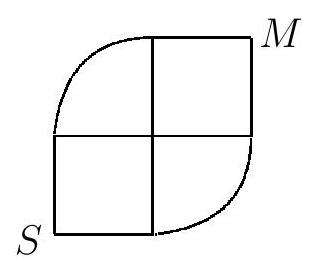
\includegraphics[max width=\textwidth, center]{2024_11_16_62d9cd06022f1460c234g-10}
\end{enumerate}

Obliczyć prawdopodobieństwo, że przejdzie przez punkt $M$, jeżeli na każdym skrzyżowaniu alejek wybiera kolejną (jeszcze nie przebytą) alejkę z tym samym prawdopodobieństwem lub kończy spacer, gdy nie ma takiej alejki.\\
4. Uczeń zna odpowiedzi na 20 spośród 30 pytań egzaminacyjnych. Na egzaminie losuje dwa pytania. Jeżeli odpowie poprawnie na oba, to egzamin zda, jeżeli na żadne, to nie zda, a jeżeli na jedno, to wynik egzaminu rozstrzyga odpowiedź na dodatkowe wylosowane pytanie. Obliczyć prawdopodobieństwo, że uczeń zda egzamin.\\
5. W trójkąt o wierzchołkach $A(-1,-1), B(3,1), C(1,3)$ wpisano kwadrat tak, że dwa jego wierzchołki leżą na boku $A B$ trójkąta. Wyznaczyć współrzędne wierzchołków kwadratu oraz stosunek pola kwadratu do pola trójkąta. Sporządzić rysunek.\\
6. Ostrosłup prawidłowy czworokątny $A B C D S$ o krawędzi podstawy $a$ ma pole powierzchni całkowitej $5 a^{2}$. Środkiem krawędzi bocznej $A S$ jest punkt $M$. Obliczyć promień kuli opisanej na ostrosłupie $A B C D M$ oraz cosinus kąta pomiędzy ścianami bocznymi $C D M$ oraz $B C M$.

\section*{PRACA KONTROLNA nr 6 - POZIOM PODSTAWOWY}
\begin{enumerate}
  \item Rozwią̇̇ równanie
\end{enumerate}

$$
2\left(\log _{2}(2-x)\right)^{2}-3 \log _{2}(2-x)-2=0
$$

\begin{enumerate}
  \setcounter{enumi}{1}
  \item Rozwiąż nierówność wykładniczą
\end{enumerate}

$$
4^{\frac{1}{2} x^{2}-x} \cdot 3^{x^{2}+7 x-2} \leqslant 9^{x^{2}+2 x} \cdot 2^{x-2}
$$

\begin{enumerate}
  \setcounter{enumi}{2}
  \item Określ dziedzinę funkcji $f(x)=\frac{-1}{1-\sqrt{5-x^{2}}}-1$. Dla jakich argumentów funkcja przyjmuje wartości ujemne?
  \item W przedziale $[0,2 \pi]$ wyznacz wszystkie liczby spełniające równanie
\end{enumerate}

$$
\operatorname{tg}^{2} x=8|\cos x|-1
$$

\begin{enumerate}
  \setcounter{enumi}{4}
  \item Oblicz pole ośmiokąta będącego wspólną częścią kwadratu o boku długości 4 oraz jego obrazu w obrocie o kąt $\frac{\pi}{4}$ względem środka kwadratu. Wyznacz promień okręgu opisanego na tym ośmiokącie i sporządź rysunek.
  \item Dane są punkty $A(0,-2)$ oraz $B(4,0)$. Wyznacz wszystkie punkty $P$ leżące na paraboli $y=x^{2}$, dla których $\triangle A B P$ jest prostokątny. Sporządź rysunek.
\end{enumerate}

\section*{PRACA KONTROLNA nr 6 - POZIOM RoZsZERZoNY}
\begin{enumerate}
  \item Liczby $a_{1}, a_{2}, \ldots, a_{n}$, gdzie $n$ jest pewną liczbą parzystą, tworzą ciąg arytmetyczny o sumie 15 . Suma wszystkich wyrazów o numerach parzystych w tym ciągu wynosi 0 , a iloczyn $a_{1} a_{2}=150$. Jakie to liczby?
  \item Rozwiąż nierówność logarytmiczną
\end{enumerate}

$$
\log _{3}\left(x^{3}-x^{2}-4 x-2\right) \leqslant \log _{\sqrt{3}} \sqrt{x+1}
$$

\begin{enumerate}
  \setcounter{enumi}{2}
  \item Rozwią̇z nierówność trygonometryczną
\end{enumerate}

$$
1-2 \sin ^{2} 2 x+4 \sin ^{4} 2 x-8 \sin ^{6} 2 x+\cdots>\frac{1}{3-2 \sin ^{2} x}
$$

której lewa strona jest sumą nieskończonego ciągu geometrycznego. Zaznacz dziedzinę i zbiór rozwiązań nierówności na kole trygonometrycznym.\\
4. Kwadrat o boku długości 4 obrócono o kąt $\frac{\pi}{6}$ względem środka kwadratu, w kierunku przeciwnym do ruchu wskazówek zegara. Oblicz pole wspólnej części kwadratu wyjściowego i jego obrazu w tym obrocie. Sporządź rysunek.\\
5. Wyznacz równania tych stycznych do okręgu $x^{2}+y^{2}=1$, które w przecięciu z okręgiem $x^{2}-16 x+y^{2}+39=0$ tworzą cięciwy długości 8 . Sporządź rysunek.\\
6. Wyznacz i narysuj funkcję $g(m)$ określającą liczbę rozwiązań równania

$$
(m-1) \frac{1}{4^{x}}+(m+1) 2^{1-x}=2-m
$$

w zależności od rzeczywistego parametru $m$.

\section*{PRACA KONTROLNA nr 7 - POZIOM PODSTAWOWY}
\begin{enumerate}
  \item Rozwiązać nierówność $\frac{1}{|x-1|} \leqslant x+3$ i podać jej interpretację graficzną.
  \item W przedziale $[0,2 \pi]$ rozwiązać nierówność $2 \sin ^{2} x>1+\cos x$. Zbiór rozwiązań zaznaczyć na kole trygonometrycznym.
  \item Znaleźć równanie okręgu stycznego do obu osi układu współrzędnych i do dodatniej gałęzi hiperboli $y=\frac{1}{x}$. Sporządzić rysunek.
  \item Zaznaczyć na płaszczyźnie zbiory $A=\left\{(x, y): 1-\sqrt{2|x|-x^{2}} \leqslant|y| \leqslant 1+\sqrt{2-|x|}\right\}$ oraz $B=\{(x, y):|x| \leqslant 1,|y| \leqslant 1\}$ i obliczyć pole figury $B \backslash A$.
  \item Trapez prostokątny, w którym stosunek długości podstaw wynosi $3: 2$, jest opisany na okręgu o promieniu $r$. Wyznaczyć stosunek pola koła do pola trapezu oraz cosinus kąta ostrego w tym trapezie.
  \item Płaszczyzna przechodząca przez krawędź podstawy graniastosłupa prawidłowego trójkątnego, w którym wszystkie krawędzie są równe, dzieli ten graniastosłup na dwie bryły o tej samej objętości. Znaleźć kąt nachylenia płaszczyzny do podstawy. Sporządzić rysunek.
\end{enumerate}

\section*{PRACA KONTROLNA nr 7 - POZIOM ROZSZERZONY}
\begin{enumerate}
  \item Rozwiązać nierówność $\frac{3}{x^{2}-2 x} \leqslant \frac{1}{|x|}$.
  \item W przedziale $[0,2 \pi]$ rozwiązać nierówność $\sqrt{\sin ^{2} x-\sin x} \geqslant \cos x$. Zbiór rozwiązań zaznaczyć na kole trygonometrycznym.
  \item Znaleźć i zaznaczyć na płaszczyźnie zbiór punktów $\left\{(x, y): \log _{x^{2}+y^{2}}(x+2 y) \geqslant 1\right\}$.
  \item Znaleźć równanie okręgu stycznego do osi $O x$ oraz do obu gałęzi krzywej o równaniu $y=\frac{1}{x^{2}}$. Sporządzić rysunek. Wskazówka: Skorzystać z algebraicznego warunku styczności.
  \item W trapezie opisanym na okręgu o promieniu $r$ kąt ostry przy podstawie leżący naprzeciw krótszej przekątnej ma miarę $30^{\circ}$, a krótsza przekątna tworzy z podstawą kąt $45^{\circ}$. Obliczyć obwód trapezu oraz tangens kąta pomiędzy jego przekątnymi. Sporządzić rysunek.
  \item Przez wierzchołek $S$ stożka poprowadzono płaszczyznę przecinającą jego podstawę wzdłuż cięciwy $A B$. Miara kąta $\angle A S B$ jest równa $\alpha$, a miara kąta $\angle A O B$ jest równa $\beta$, gdzie $O$ jest środkiem podstawy. Obliczyć sinus kąta rozwarcia stożka. Podać warunki rozwiązalności zadania oraz warunek, aby kąt rozwarcia stożka był kątem prostym.
\end{enumerate}

\end{document}